\documentclass[bwprint]{gmcmthesis}
\usepackage{amsmath}
\numberwithin{figure}{section}
\renewcommand{\thefigure}{\arabic{section}-\arabic{figure}} 
% \documentclass[withoutpreface,bwprint]{cumcmthesis}
% 去掉封面与编号页

\title{中国研究生数学建模竞赛论文标题}
\baominghao{No.00000001} %参赛队号
\schoolname{XX大学/学院}%学校名称
\membera{队员A} %队员A
\memberb{队员B} %队员B
\memberc{队员C} %队员C
\begin{document}
 \maketitle
 \begin{abstract}
第一段:针对自己选择的题目,说明自己用了什么方法来解决的(这类题属于哪种典型的问题),其中利用了哪些关键的算法,再说出自己的所建模型的创新点。没有创新点,也可以说自己所建的模型相比较于其它的是一个很好的方案。

第二段:问题一中,针对具体问题,进行分析和求解,几句话介绍自己是怎么解决的,有数字结果的也可以直接贴结果。

第三段:问题二中,类比于第二段。

第四段:问题三中,类比于第三段。

第五段:问题四中,类比于第四段。

第六段:如果有问题五,类比于第五段,没有就结束,也可以写一下团队的想法。






\keywords{针对具体的问题列一到两个关键字\quad  建模算法列出\quad }
\end{abstract}

%\pagestyle{plain}

%目录
\tableofcontents

\section{问题背景与问题重述}
\subsection{问题背景}
2019年底爆发的新冠肺炎疫情给全人类带来深重苦难,至今已有4亿多人感染,6000多万人死亡。面对突如其来的疫情,中国政府始终将人民生命财产安全放在第一位,果断采取科学防控措施,有效遏制了疫情大面积蔓延,有力改变了病毒传播的危险进程,最大限度保护了人民生命安全和身体健康。直至2022年初,我国的新冠肺炎疫情已得到基本控制。
\par 然而,在2022年3月上海突然爆发了奥密克戎疫情,直到现在疫情仍未得到根本控制,使得疫情防控态势又紧张了起来。面对疫情,需要我们采取科学防控措施,利用已经公布的相关数据和数学模型,对本轮上海新冠肺炎疫情进行预测,使人们更好的认识新冠肺炎传播规律,也能为相关部门采取防控措施提供参考,对疫情防控具有积极作用。

\subsection{问题重述}
题目提示需要在分析上海市卫生健康委员会和国家卫生健康委员会通报的实时疫情数据的基础上(主要包括累计报告病例、累计治愈病例、累计死亡病例、跟踪隔离人数、单日新增确诊病例等),建立新冠肺炎传播模型以预测未来疫情发展趋势并评估防疫策略。
\begin{enumerate}
\item
问题1:搜集有关美国国内疫情应对措施,分析在此防控措施下造成的美国疫情蔓延态势。若上海采取相同防控措施,通过建立模型分析疫情蔓延情况及可能带来的严重后果。
\item 问题2:疫情爆发初期,上海市政府采取精准防控策略并公布了相关数据,需要分析上述数据以建立数学模型预测在该措施下的再生数。通过前面建立的模型预测两个月内疫情发展趋势和累计病例数。
\item 问题3:随着疫情发展趋势,上海市政府加强了管控措施,积极推行如:全员核算、启用方舱医院接收轻型患者和无症状感染者等措施。需要根据对应的公布数据,建立恰当的数学模型预测包括:流行时间、流行规模等指标在内的本次疫情发展趋势。预测完成后还需要根据五月份的数据来验证模型的有效性。若上海疫情在五月中旬之后仍未结束,需要根据模型预测一周内疫情发展趋势。
\item 问题4:根据建模结果,总结出一些对抗击疫情有积极作用的针对性建议,给有关部门进行参考。
\end{enumerate}

\begin{figure}[!h]
\centering
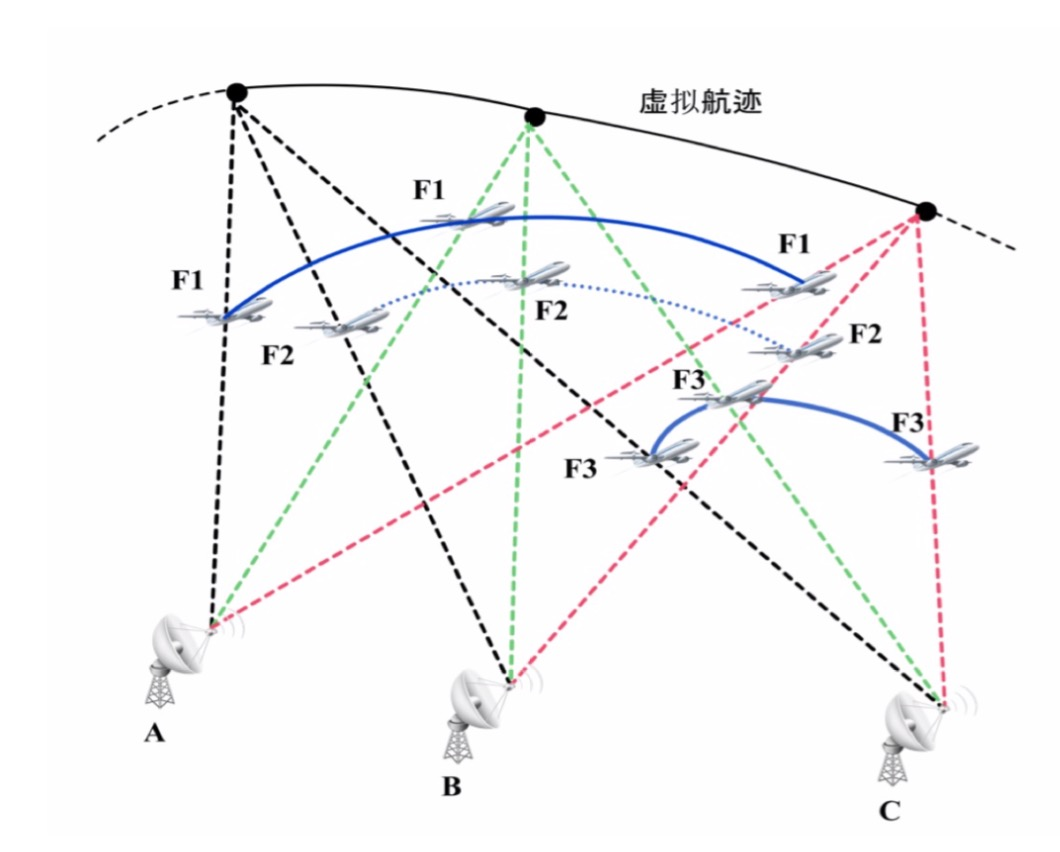
\includegraphics[width=.7\textwidth]{test.jpg}
\caption{对雷达实施距离多假目标欺骗干扰示意图}
\label{fig1}
\end{figure}


\section{模型假设}
\begin{enumerate}
\item 假设气候因素(温度、湿度)对病毒传播无影响
\item 假设人口总数在预测区间内恒定
\item 假设个体对病毒的易感性相同
\item 假设病毒传染性不变
\end{enumerate}
\begin{figure}[!h]
\centering
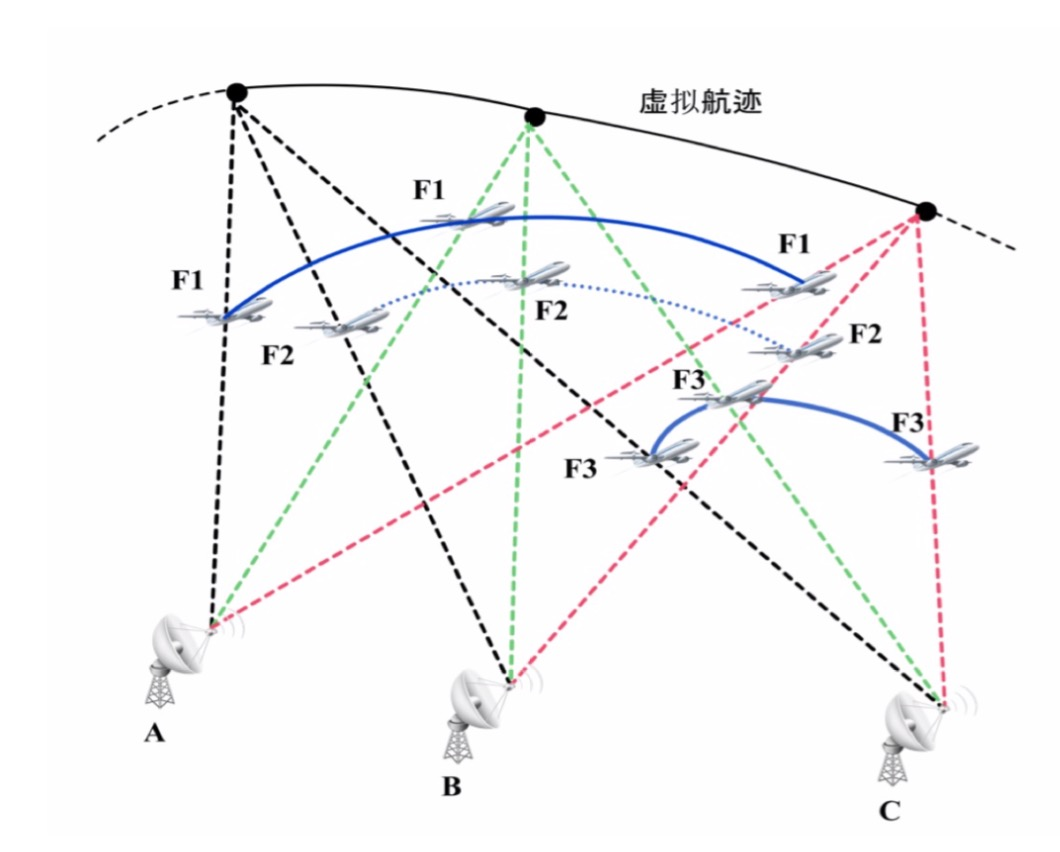
\includegraphics[width=.7\textwidth]{test.jpg}
\caption{对雷达实施距离多假目标欺骗干扰示意图}
\label{fig1}
\end{figure}




\section{符号说明}
\begin{tabular}{cc}
 \hline
 \makebox[0.4\textwidth][c]{符号}	&  \makebox[0.5\textwidth][c]{意义} \\ \hline
    $\lambda_a$	    & 宽度(cm) \\ \hline
    $\beta$	    & 宽度(cm) \\ \hline
    $\phi$	    & 宽度(cm) \\ \hline
    $r_a$	    & 宽度(cm) \\ \hline
    $M$	    & 宽度(cm) \\ \hline
    $\beta$	    & 宽度(cm) \\ \hline
    $\beta$	    & 宽度(cm) \\ \hline
    $\beta$	    & 宽度(cm) \\ \hline
 	L	           & 长度(cm)  \\ \hline
\end{tabular}
\section{问题一的分析与求解}
假设在疫情爆发初期,上海市政府采取美国的防疫策略,请建立数学模型预测本次疫情在两个月内的发展趋势和累计病例数
\subsection{问题分析}
分为随机(Stochastic)模型和决定性(Deterministic)模型
\subsection{隔间模型}
隔间模型是一种疾病传播模型,把人群分为
\subsection{参数辨识}
优化算法,拟合得到参数
\subsection{数据收集与预处理}
\begin{equation}
\frac{dS}{dt}=-\frac{\beta SI}{N}\\
\end{equation}
\begin{equation}
\frac{dI}{dt}=\frac{\beta SI}{N}-\frac{I}{D}\\
\end{equation}
\begin{equation}
\frac{dR}{dt}=\frac{I}{D}
\end{equation}
\subsection{小结}


\section{问题二的分析与求解}
请根据上海市政府初期的精准防控策略和对应的公布数据,建立数学模型估计在该防控策略下的再生数。进一步,如果上海市政府一直执行初期精准防控的策略,请根据模型预测本次疫情在两个月内的发展趋势和累计病例数
\subsection{问题分析}
SEIR模型
机器学习方法,时间序列方法
缺乏可解释性
\subsection{再生数}
\subsection{SLIRS模型}
SLIRS模型,将人群分成了
\par 采用随机模型,符合二项分布。对每一个个体,其
\subsection{考虑大规模疫苗接种的模型}


\section{问题三的分析与求解}
随后,上海市政府根据疫情的发展趋势加强了管控措施,如全员核酸、启用了方舱医院接收轻型患者和无症状感染者等, 请根据对应的公布数据,建立数学模型预测本次疫情的发展趋势,包括流行时间、流行规模等,并利用4月30日后公布的数据验证模型有效性。若上海市疫情在5月16日后尚未结束,请根据模型预测一周内的疫情发展趋势
\subsection{问题分析}



\section{给上海市政府的建议信}


\section{模型的评价}
\subsection{模型的优点}
模型的优点模型的优点模型的优点模型的优点模型的优点模型的优点模型的优点模型的优点模型的优点模型的优点模型的优点模型的优点模型的优点模型的优点。
\subsection{模型的缺点}
模型的缺点模型的缺点模型的缺点模型的缺点模型的缺点模型的缺点模型的缺点模型的缺点模型的缺点模型的缺点模型的缺点模型的缺点模型的缺点模型的缺点。



\section{写作参考格式}
写作过程中可能要用到一些格式参考,正式写作的时候,可以直接将这一章删掉即可。

\textbf{无序列表格式}
\begin{itemize}
\item 无序列表1
\item 无序列表2
\item 无序列表3
\item 无序列表4
\end{itemize}


\textbf{表格格式}

\begin{tabular}{cc}
 \hline
 \makebox[0.4\textwidth][c]{符号}	&  \makebox[0.5\textwidth][c]{意义} \\ \hline
 D	    & 宽度(cm) \\ \hline
 L	    & 长度(cm)  \\ \hline
\end{tabular}


%
%\textbf{图片格式}
%\begin{figure}[h]
%\centering
%\includegraphics[width=5cm]{xxx.jpg}
%\caption{图片标题}
%\end{figure}

\section{参考文献}
%参考文献
\begin{thebibliography}{1.2}%宽度9
\setlength{\itemsep}{-2mm}
 \bibitem{bib:one} 
 韩中庚. 数学建模方法及其应用[M]. 高等教育出版社, 2005.
 \bibitem{bib:two}
 韩中庚. 数学建模方法及其应用[M]. 高等教育出版社, 2005.
  \bibitem{bib:two}
 韩中庚. 数学建模方法及其应用[M]. 高等教育出版社, 2005.
\end{thebibliography}

\newpage
%附录
\appendix
\section{程序代码}
%设置不同语言即可。
\begin{lstlisting}[language=Matlab] 
kk=2;[mdd,ndd]=size(dd);
while ~isempty(V)
[tmpd,j]=min(W(i,V));tmpj=V(j);
for k=2:ndd
[tmp1,jj]=min(dd(1,k)+W(dd(2,k),V));
tmp2=V(jj);tt(k-1,:)=[tmp1,tmp2,jj];
end
tmp=[tmpd,tmpj,j;tt];[tmp3,tmp4]=min(tmp(:,1));
if tmp3==tmpd, ss(1:2,kk)=[i;tmp(tmp4,2)];
else,tmp5=find(ss(:,tmp4)~=0);tmp6=length(tmp5);
if dd(2,tmp4)==ss(tmp6,tmp4)
ss(1:tmp6+1,kk)=[ss(tmp5,tmp4);tmp(tmp4,2)];
else, ss(1:3,kk)=[i;dd(2,tmp4);tmp(tmp4,2)];
end;end
dd=[dd,[tmp3;tmp(tmp4,2)]];V(tmp(tmp4,3))=[];
[mdd,ndd]=size(dd);kk=kk+1;
end; S=ss; D=dd(1,:);
 \end{lstlisting}


\end{document} 